\documentclass[oneside]{uffstex}
\usepackage[utf8]{inputenc}
\usepackage[utf8]{inputenc}
\usepackage[T1]{fontenc}
\usepackage{float}
\usepackage{emptypage}
\usepackage[table]{xcolor}
\usepackage{tikz}
\usepackage[style=abnt-numeric]{biblatex}
\addbibresource{refs.bib}
%======================CAPA========================

\titulo{Implementação de Blackjack}
\subtitulo{SISTEMAS DIGITAIS}
\autor{docente: GEOMAR ANDRE SCHREINER \\discentes: ARTHUR EMANUEL DA SILVA (2211100029)\\ E JÉSSICA BRITO DA SILVA (20240002517)}
\curso{Ciência da Computação}
\cidade{Chapecó}
\uf{SC}
%==========PALAVRAS CHAVE =======
\palavrachave{palavra chave}
\palavrachave{palavra chave}
\palavrachave{palavra chave}

\begin{document}
\imprimircapa%

%===============================SUMARIO===================================%
\pdfbookmark{\contentsname}{toc}
\tableofcontents*
\cleardoublepage%

\textual%
\chapter{Introdução}
\section{Resumo} 
Este relatório descreve o projeto e a implementação de uma Máquina de Estados Finitos (FSM) em VHDL para um jogo de Blackjack simplificado, executado em uma placa FPGA DE1 - Cyclone II. O sistema gerencia as regras do jogo para um jogador e um carteador, incluindo distribuição de cartas, decisões de "HIT" e "STAY", e determinação do vencedor. Uma FSM secundária foi desenvolvida para a geração de cartas em modos aleatório ou manual. A interação do jogador é feita por botões físicos (HIT, STAY, START), com o botão START funcionando também como reset. As pontuações e cartas são exibidas em displays de 7 segmentos. O projeto foi desenvolvido em VHDL e implementado fisicamente em uma FPGA, validando seu funcionamento conforme o esperado, demonstrando a aplicação de design digital em hardware reconfigurável.
\section{Descrição da aplicação}
O jogo de Blackjack envolve um jogador e um carteador, com o objetivo de obter uma mão de cartas com pontuação superior à do adversário, sem ultrapassar 21 pontos. As regras incluem a distribuição inicial de duas cartas para cada participante , opções de "HIT" (pedir carta) ou "STAY" (manter a mão) para o jogador , e uma lógica automática para o carteador (pedir carta se a mão for menor que 17, e parar com 17 ou mais). A pontuação das cartas segue o padrão do jogo, com figuras valendo 10 e Ás valendo 1 ou 11 pontos.
A arquitetura do sistema compreende duas Máquinas de Estados Finitos (FSMs) principais: uma para o controle do fluxo do jogo (blackjack)  e outra para a geração e seleção de cartas (Random ou manual, para caso de testes). As entradas do sistema incluem botões para as ações do jogador (HIT, STAY, START), sendo o START também responsável pelo reset. As saídas compreendem indicadores de status do jogo (WIN, LOSE, TIE) e displays de 7 segmentos para a carta atual (em hexadecimal) e a soma total da mão do jogador (em decimal). Este trabalho visa demonstrar a aplicação prática de VHDL e FSMs no desenvolvimento de um sistema interativo em ambiente FPGA.

\chapter{Estratégia de resolução}
Para implementar em VHDL o jogo de Blackjack, utilizamos como resolução duas máquinas de estados finitas (finite state machine - FSM) que atuam em conjunto para a realização das rodadas do jogo. Em uma das FSM, reside a lógica para gerar e apresentar cartas que podem ser aleatórias ou manualmente colocadas, enquanto na segunda máquina está inserida a lógica por trás do estouro (isto é, a soma das cartas ultrapassar 21) ou a possível comparação das somas de mãos caso ambos carteador e jogador tenham escolhido enviar um sinal de STAY e o programa não tenha uma resposta imediata para um vencedor.
\section{FSM - Gerador de cartas}
Em primeiro lugar, construímos uma máquina de estados finita com objetivo de gerar cartas que podem ser aleatórias para os casos de implementação dinâmica do jogo ou manuais, exclusiva para casos de testagem relacionadas a acurácia do programa em VHDL. O comportamento do gerador de cartas pode ser observado na esquemática construída abaixo:
\begin{center}
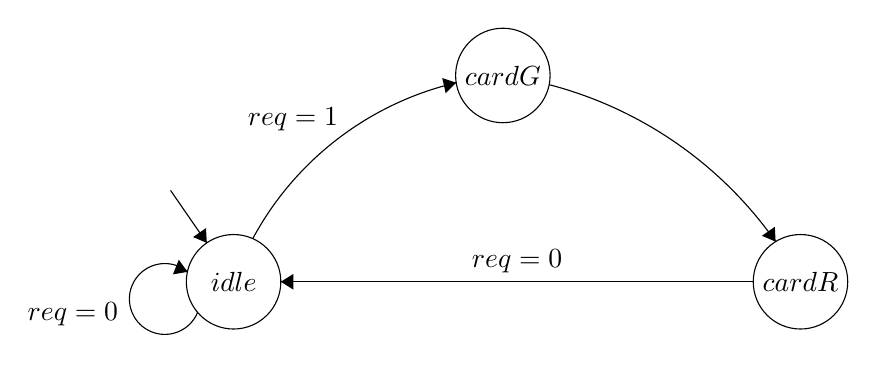
\begin{tikzpicture}[scale=0.2]
\tikzstyle{every node}+=[inner sep=0pt]
\draw [black] (23,-29.8) circle (3);
\draw (23,-29.8) node {$idle$};
\draw [black] (40.1,-16.7) circle (3);
\draw (40.1,-16.7) node {$cardG$};
\draw [black] (59,-29.8) circle (3);
\draw (59,-29.8) node {$cardR$};
\draw [black] (20.721,-31.733) arc (-21.96376:-309.96376:2.25);
\draw (15.69,-31.89) node [left] {$req=0$};
\fill [black] (20.08,-29.17) -- (19.52,-28.4) -- (19.15,-29.33);
\draw [black] (24.218,-27.061) arc (151.69126:103.21888:19.826);
\fill [black] (37.14,-17.16) -- (36.25,-16.86) -- (36.47,-17.83);
\draw (26.77,-20.23) node [above] {$req=1$};
\draw [black] (43.041,-17.284) arc (75.39272:35.15395:25.433);
\fill [black] (57.42,-27.25) -- (57.37,-26.31) -- (56.55,-26.88);
\draw [black] (56,-29.8) -- (26,-29.8);
\fill [black] (26,-29.8) -- (26.8,-30.3) -- (26.8,-29.3);
\draw (41,-29.3) node [above] {$req=0$};
\draw [black] (19,-24) -- (21.3,-27.33);
\fill [black] (21.3,-27.33) -- (21.25,-26.39) -- (20.43,-26.96);
\end{tikzpicture}
\end{center}
A máquina de estados para o gerador de cartas foi projetada de forma que o sinal reqManual seja usado apenas para testes de funcionalidade. Em uma condição de jogo normal, o reqManual estará sempre em '0'. Quando o sinal req é ativado a partir do estado idle, o sistema decide ir para o CardG, onde uma carta será criada de forma aleatória (reqManual = 0) ou inserida manualmente. No próximo ciclo de clock, essa carta será lida no estado read e então enviada como entrada para a FSM principal que gerencia o jogo.
\section{Diagrama de transição do gerador de cartas}
Para detalhar o comportamento da máquina de estados do gerador de cartas, a tabela abaixo mostra como ela transita entre os diferentes estados. Essa tabela define as regras para o funcionamento do programa em VHDL, com base nos sinais de entrada.
\begin{table}[H]
    \centering
    \caption{DIAGRAMA DE PRÓXIMO ESTADO}
    \begin{tabular}{|p{2cm}|p{1cm}|p{2cm}|p{1.25cm}|}
        \hline
        CURRENT & req & reqManual & NEXT \\ 
        \hline
        idle & 0 & x & idle  \\
        \hline
        idle & 1 & x & CardG  \\
        \hline
        CardG & 0 & x & idle  \\
        \hline
    \end{tabular}
    \label{tab:geradorcarta}
\end{table}
A tabela acima descreve as transições de estado para a FSM do gerador de cartas. Ela explica como o sistema se move dentro de um estado CURRENT, utilizando os sinais req e reqManual. O modo reqManual é prioritário para testar diferentes cenários, enquanto um req em '0' faz a FSM voltar para o estado idle. O estado read indica quando a carta está pronta para ser utilizada pelo restante do sistema.

\section{FSM - Execução do jogo Blackjack}

A projeção da segunda máquina de estados seguiu à risca as recomendações dadas pelo problema, ciente das limitações apresentadas para a execução do jogo na FPGA. Dessa forma, a proposta escolhida foi que o player jogue até que haja um estado de BUST ou STAY, passando a vez para o dealer que decide de forma automatizada se transita para um estado de HIT ou STAY. O jogo se inicia com a distribuição obrigatória de duas cartas, que não tem qualquer tipo de condição para serem dadas. A partir da soma de ambas, o jogador ou carteador decide no estado de TURN se deseja solicitar outra carta ou parar o jogo com o sinal de STAY.

\begin{center}
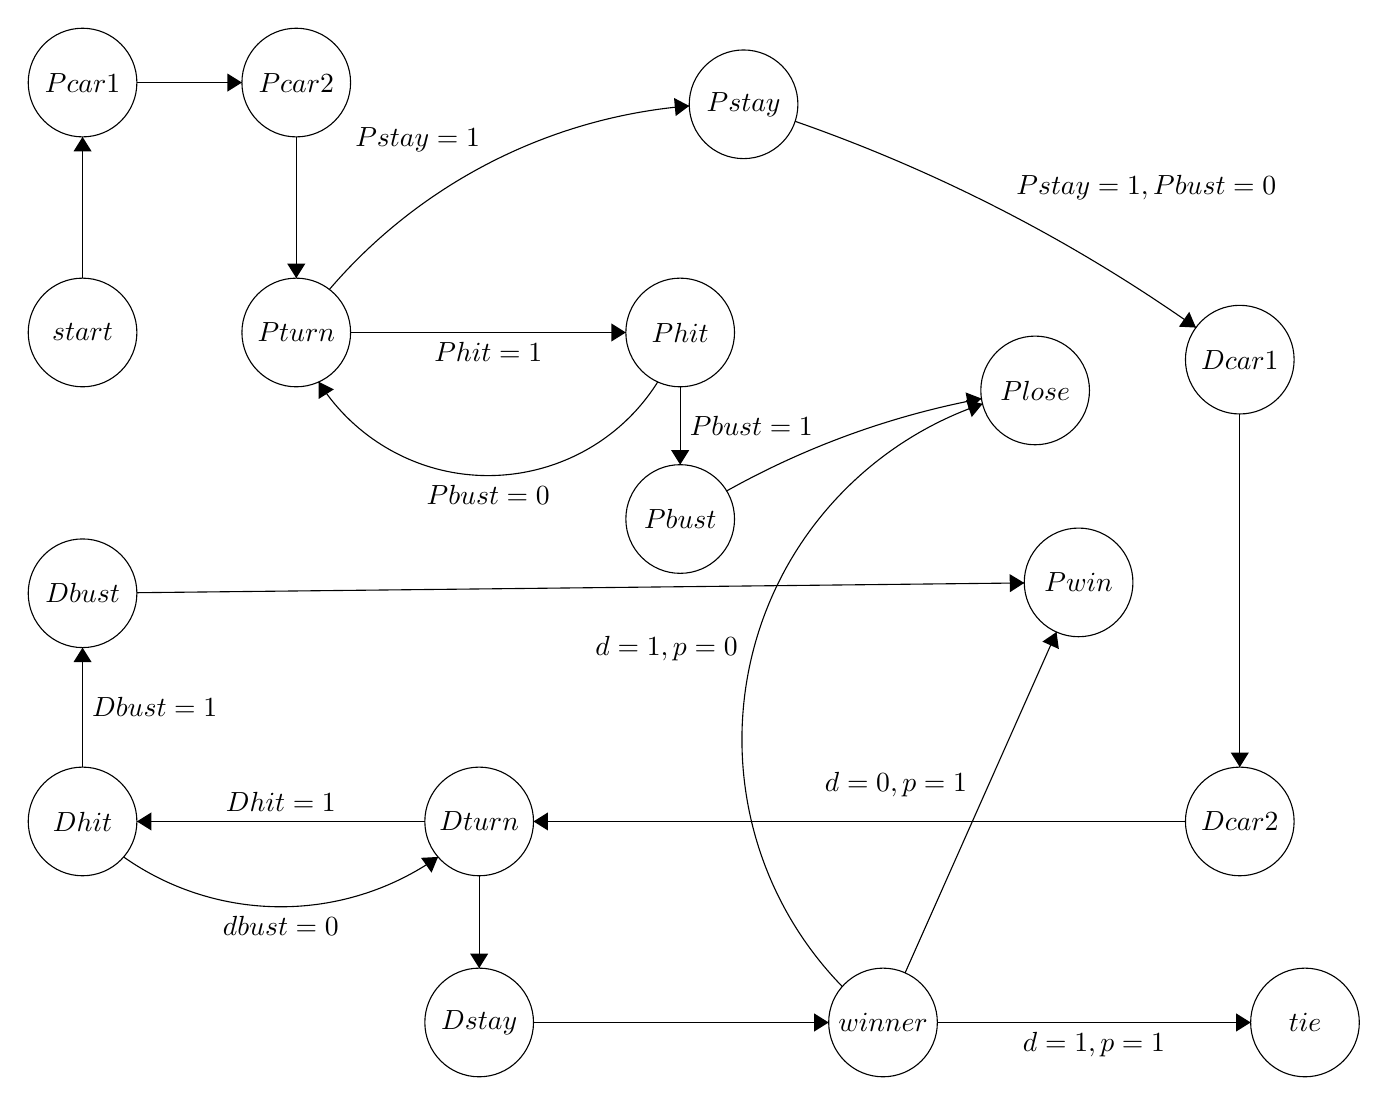
\begin{tikzpicture}[scale=0.23]
\tikzstyle{every node}+=[inner sep=0pt]
\draw [black] (6.6,-17.8) circle (3);
\draw (6.6,-17.8) node {$start$};
\draw [black] (6.6,-4) circle (3);
\draw (6.6,-4) node {$Pcar1$};
\draw [black] (18.4,-4) circle (3);
\draw (18.4,-4) node {$Pcar2$};
\draw [black] (18.4,-17.8) circle (3);
\draw (18.4,-17.8) node {$Pturn$};
\draw [black] (43.1,-5.2) circle (3);
\draw (43.1,-5.2) node {$Pstay$};
\draw [black] (39.6,-17.8) circle (3);
\draw (39.6,-17.8) node {$Phit$};
\draw [black] (39.6,-28.1) circle (3);
\draw (39.6,-28.1) node {$Pbust$};
\draw [black] (59.2,-21) circle (3);
\draw (59.2,-21) node {$Plose$};
\draw [black] (70.5,-19.3) circle (3);
\draw (70.5,-19.3) node {$Dcar1$};
\draw [black] (70.5,-44.8) circle (3);
\draw (70.5,-44.8) node {$Dcar2$};
\draw [black] (28.5,-44.8) circle (3);
\draw (28.5,-44.8) node {$Dturn$};
\draw [black] (6.6,-44.8) circle (3);
\draw (6.6,-44.8) node {$Dhit$};
\draw [black] (28.5,-55.9) circle (3);
\draw (28.5,-55.9) node {$Dstay$};
\draw [black] (6.6,-32.2) circle (3);
\draw (6.6,-32.2) node {$Dbust$};
\draw [black] (61.6,-31.6) circle (3);
\draw (61.6,-31.6) node {$Pwin$};
\draw [black] (50.8,-55.9) circle (3);
\draw (50.8,-55.9) node {$winner$};
\draw [black] (74.1,-55.9) circle (3);
\draw (74.1,-55.9) node {$tie$};
\draw [black] (6.6,-14.8) -- (6.6,-7);
\fill [black] (6.6,-7) -- (6.1,-7.8) -- (7.1,-7.8);
\draw [black] (9.6,-4) -- (15.4,-4);
\fill [black] (15.4,-4) -- (14.6,-3.5) -- (14.6,-4.5);
\draw [black] (18.4,-7) -- (18.4,-14.8);
\fill [black] (18.4,-14.8) -- (18.9,-14) -- (17.9,-14);
\draw [black] (20.23,-15.425) arc (139.44181:94.61239:29.252);
\fill [black] (40.1,-5.29) -- (39.26,-4.85) -- (39.35,-5.85);
\draw (25.1,-7.87) node [above] {$Pstay=1$};
\draw [black] (21.4,-17.8) -- (36.6,-17.8);
\fill [black] (36.6,-17.8) -- (35.8,-17.3) -- (35.8,-18.3);
\draw (29,-18.3) node [below] {$Phit=1$};
\draw [black] (39.6,-20.8) -- (39.6,-25.1);
\fill [black] (39.6,-25.1) -- (40.1,-24.3) -- (39.1,-24.3);
\draw (40.1,-22.95) node [right] {$Pbust=1$};
\draw [black] (42.168,-26.55) arc (119.25474:100.57058:46.085);
\fill [black] (56.24,-21.45) -- (55.36,-21.11) -- (55.54,-22.09);
\draw [black] (45.948,-6.141) arc (70.76112:54.77831:89.511);
\fill [black] (68.08,-17.53) -- (67.71,-16.66) -- (67.14,-17.48);
\draw (65.34,-10.53) node [above] {$Pstay=1,Pbust=0$};
\draw [black] (70.5,-22.3) -- (70.5,-41.8);
\fill [black] (70.5,-41.8) -- (71,-41) -- (70,-41);
\draw [black] (67.5,-44.8) -- (31.5,-44.8);
\fill [black] (31.5,-44.8) -- (32.3,-45.3) -- (32.3,-44.3);
\draw [black] (25.5,-44.8) -- (9.6,-44.8);
\fill [black] (9.6,-44.8) -- (10.4,-45.3) -- (10.4,-44.3);
\draw (17.55,-44.3) node [above] {$Dhit=1$};
\draw [black] (28.5,-47.8) -- (28.5,-52.9);
\fill [black] (28.5,-52.9) -- (29,-52.1) -- (28,-52.1);
\draw [black] (38.366,-20.524) arc (-32.13477:-147.86523:11.061);
\fill [black] (19.63,-20.52) -- (19.64,-21.47) -- (20.48,-20.94);
\draw (29,-26.2) node [below] {$Pbust=0$};
\draw [black] (6.6,-41.8) -- (6.6,-35.2);
\fill [black] (6.6,-35.2) -- (6.1,-36) -- (7.1,-36);
\draw (7.1,-38.5) node [right] {$Dbust=1$};
\draw [black] (9.6,-32.17) -- (58.6,-31.63);
\fill [black] (58.6,-31.63) -- (57.79,-31.14) -- (57.81,-32.14);
\draw [black] (31.5,-55.9) -- (47.8,-55.9);
\fill [black] (47.8,-55.9) -- (47,-55.4) -- (47,-56.4);
\draw [black] (48.552,-53.918) arc (-135.78684:-251.27913:19.567);
\fill [black] (56.3,-21.74) -- (55.38,-21.52) -- (55.7,-22.47);
\draw (42.8,-35.26) node [left] {$d=1,p=0$};
\draw [black] (52.02,-53.16) -- (60.38,-34.34);
\fill [black] (60.38,-34.34) -- (59.6,-34.87) -- (60.51,-35.28);
\draw (55.47,-42.76) node [left] {$d=0,p=1$};
\draw [black] (53.8,-55.9) -- (71.1,-55.9);
\fill [black] (71.1,-55.9) -- (70.3,-55.4) -- (70.3,-56.4);
\draw (62.45,-56.4) node [below] {$d=1,p=1$};
\draw [black] (26.235,-46.76) arc (-54.83515:-125.16485:15.08);
\fill [black] (26.23,-46.76) -- (25.29,-46.81) -- (25.87,-47.63);
\draw (17.55,-50.01) node [below] {$dbust=0$};
\end{tikzpicture}
\end{center}
Observa-se que só transitamos ao estado de WINNER quando ambos carteador e jogador enviam o sinal de STAY, no cenário em que o jogo teria acabado sem nenhum dos dois terem ultrapassado 21 na soma de suas cartas. Essa comparação está implicita na máquina de estados e o resultado dela é o sinal '1' que simboliza qual dos dois tem o maior somatório em mãos, ou ainda '1' para ambos carteador e jogador caso possuem a mesma soma, configurando um empate. A única outra possibilidade de empate é o cenário onde ambos jogador e carteador ultrapassam a soma de 21 pontos.

\section{Diagrama de transição das rodadas do jogo}
Como citado anteriormente, a lógica de transição do jogo foi alinhada às limitações do ambiente de execução, seguindo todo o possível para ainda ser fielmente um jogo de Blackjack. A Tabela \ref{tab:blackjack} detalha o comportamento da Máquina de Estados Finitos (FSM) principal do jogo. Vale ressaltar que, para otimização e controle preciso do fluxo de dados, há um estado temporário (dummy) omitido na representação visual da máquina de estados, localizado imediatamente antes dos estados de obtenção de carta. Este estado intermediário é crucial para sincronizar a requisição e a leitura da carta com a máquina de geração, garantindo que a lógica da FSM principal opere apenas com cartas válidas já disponibilizadas.

\begin{table}[H]
    \centering
    \caption{DIAGRAMA DE PRÓXIMO ESTADO}
    \begin{tabular}{|p{2cm}|p{1cm}|p{1cm}|p{1cm}|p{1cm}|p{1cm}|p{1cm}|p{1cm}|p{1cm}|p{1.25cm}|}
        \hline
        CURRENT & Phit & Pstay & Pbust & Dhit & Dstay & Dbust & p & d & NEXT \\ 
        \hline
        start & x & x & x & x & x & x & x & x & Pcar1  \\
        \hline
        Pcar1 & x & x & x & x & x & x & x & x & Pcar2  \\
        \hline
        Pcar2 & x & x & x & x & x & x & x & x & Pturn  \\
        \hline
        Pturn & 1 & 0 & 0 & x & x & x & x & x & Phit  \\ 
        \hline
        Phit & x & x & 0 & x & x & x & x & x & Pturn  \\
        \hline
        Phit & x & 0 & 1 & x & x & x & x & x & Pbust  \\
        \hline
        Pbust & x & x & x & x & x & x & 0 & 1 & Plose  \\
        \hline
        %aaaaaaaaaaaaaaaa
        Pstay & 0 & 1 & 0 & x & x & x & x & x & Dcar1  \\
        \hline
        Dcar1 & x & x & x & x & x & x & x & x & Dcar2  \\
        \hline
        Dcar2 & x & x & x & x & x & x & x & x & Dturn  \\
        \hline
        Dturn & x & x & x & 1 & 0 & 0 & x & x & Dhit  \\ 
        \hline
        Dhit & x & x & x & x & x & 0 & x & x & Dturn  \\
        \hline
        Dhit & x & 0 & 1 & x & x & 1 & x & x & Dbust  \\
        \hline
        Dbust & x & x & x & x & x & x & 0 & 1 & Pwin  \\
        \hline
        Dhit & x & x & x & 0 & 1 & 0 & x & x & winner  \\
        \hline
        winner & x & x & x & x & x & x & 1 & 0 & Pwin  \\
        \hline
        winner & x & x & x & x & x & x & 0 & 1 & Plose  \\
        \hline
        winner & x & x & x & x & x & x & 0 & 0 & tie  \\
        \hline
        winner & x & x & x & x & x & x & 1 & 1 & tie  \\
        \hline
    \end{tabular}
    \label{tab:blackjack}
\end{table}
A tabela acima detalha as transições de estado para a FSM principal do Blackjack. Ela descreve como o jogo avança ao longo de um estado CURRENT, baseado nas ações do jogador (Phit, Pstay) e do dealer (Dhit, Dstay), bem como nos resultados do jogo (Pbust, Dbust, p, d). Essa formalização é essencial para a implementação precisa do fluxo de jogo em VHDL, garantindo que todas as regras e condições de vitória, derrota ou empate sejam corretamente representadas e executadas.
\section{Interação entre as máquinas de estado do problema}
A complexidade de um sistema como o Blackjack em um ambiente de FPGA exige uma abordagem modular, onde diferentes funcionalidades são delegadas a FSMs específicas. Neste projeto, a máquina de estados para o gerador de cartas funciona como um subsistema fundamental, fornecendo as cartas necessárias para a FSM principal que orquestra o jogo de Blackjack. A saída do gerador de cartas funcionará como entrada para a segunda máquina de estados, onde o jogo Blackjack efetivamente é executado.


O mecanismo de comunicação entre essas duas FSMs é iniciado pelo sinal de 'req'. Este sinal é ativado pela máquina de estados do Blackjack quando há a necessidade de uma nova carta, seja para a distribuição inicial ou para uma jogada de 'HIT' tanto do jogador quanto do dealer. Ao acionar 'req', a FSM do Blackjack entra em um estado temporário — o já mencionado "estado dummy" — que não é explicitamente representado no diagrama visual para manter a clareza e legibilidade. Uma vez que a carta é disponibilizada, a FSM do Blackjack prossegue com suas transições de estado, avaliando a nova pontuação da mão e decidindo, por exemplo, se ocorreu um "bust" (estouro de 21) ou se a jogada pode continuar, garantindo uma sincronização eficiente e segura entre as duas entidades.
\chapter{Resolução}
\section{Fase de planejamento}
Para a implementação do Blackjack, utilizamos o modelo proposto pelo exercício e que, no caso das máquinas de estado que construímos, se deu da seguinte maneira:
\begin{figure}[H]
    \centering
    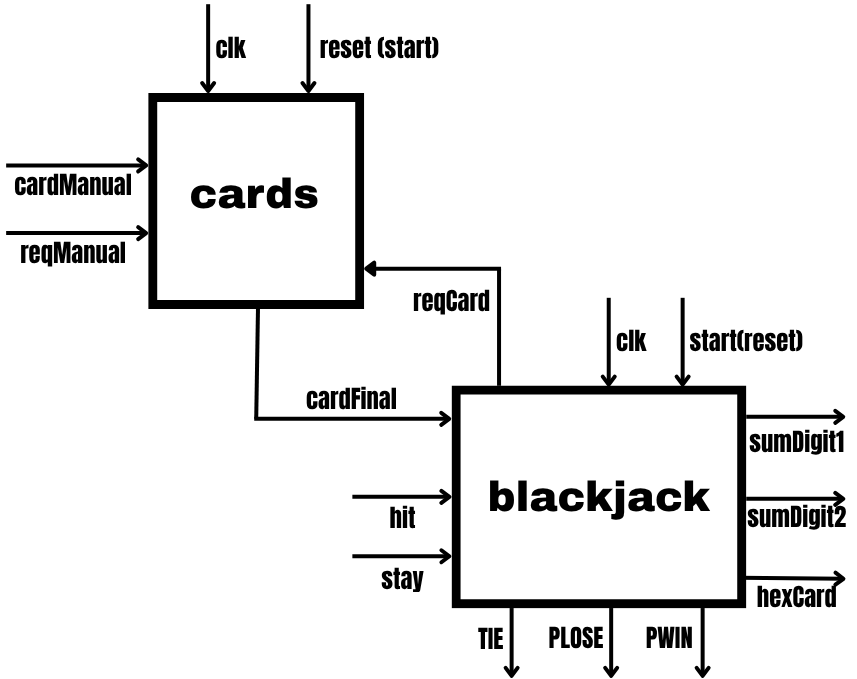
\includegraphics[width=1.0\linewidth]{planejamento_cards_blackjack.png}
    \caption{Planejamento da resolução}
    \label{fig:cards_blackjack}
\end{figure}
As máquinas cards e blackjack interagem a partir dos sinais de req e da carta gerada. Quando o sinal de req é enviado pela máquina \ref{tab:blackjack}, a máquina \ref{tab:geradorcarta} transita para o estado de cardG onde a carta será gerada. Enquanto isso, a máquina blackjack transita para o estado dummy para termos certeza de que ela receberá uma carta válida para dar prosseguimento ao jogo. Uma vez que a carta é enfim gerada, a máquina cards retorna a carta (um numero de 1-13) e a máquina blackjack agora consegue fazer alterações no somatório dos jogadores e conferir as possibilidades de estouro, de acordo com essa carta válida gerada pela outra máquina.
\section{Entidade cards}
Para a primeira máquina de estados vista na Tabela \ref{tab:geradorcarta}, utilizamos uma entidade cards que gera um número aleatório a partir de uma SEED fixa ou colocar na saida cardFinal o valor armazenado na entrada cardManual caso o reqManual esteja ativo.
\begin{figure}[H]
    \centering
    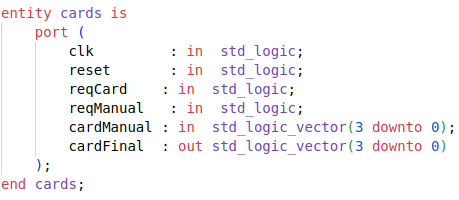
\includegraphics[width=0.8\linewidth]{cards.png}
    \caption{Entidade geradora de cartas}
    \label{fig:cards_entity}
\end{figure}
Para a entidade cards, clk representa o clock (mesmo clock recebido pela FSM2), reset retorna a máquina imediatamente para o estado de idle (mesmo sinal conectado ao START da FSM2), reqCard é o sinal recebido pela FSM2 que define a transição de blackjack de idle para cardG, reqManual define se a cartaFinal será um número aleatório ou o valor de input colocado pelo cardManual e, por fim, cardFinal é a carta que enviamos para a máquina Blackjack, que fará operações a partir dessa carta recebida para atualizar os valores do player e dealer a partir dessa entrada.
\section{Entidade Blackjack}
No caso da segunda máquina de estados vista na Tabela \ref{tab:blackjack}, utilizamos uma entidade blackjack que faz alterações em seus sinais playerValue e dealerValue de acordo com as cartas recebidas pela FSM \ref{tab:geradorcarta}. Essa entidade é responsável por receber essas cartas e realizar operações que garantem o funcionamento dentro das regras do jogo. Aqui está situada toda a lógica de vitória, derrota, estouro e tratamento de casos excepcionais (i.e estouros com Áses na mão).

\begin{figure}[H]
    \centering
    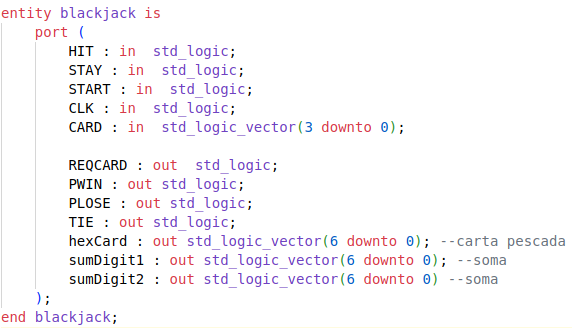
\includegraphics[width=0.9\linewidth]{blackjack.png}
    \caption{Entidade executora do jogo}
    \label{fig:blackjack_entity}
\end{figure}

Como mencionado anteriormente, os sinais de CLK e START(reset) são divididos entre as duas máquinas, o sinal de HIT leva o req para 1, dando início ao processo de gerar a carta para o jogo, STAY faz com que o jogador ou dealer pare de puxar cartas a fim de evitar o estouro, CARD é a carta recebida pela FSM1, PWIN/PLOSE/TIE são os estados de resultado do jogo, que podem ser atingidos por meio de diferentes condições definidas na arquitetura da Blackjack e, por mim, as saídas de display exibem a última carta pescada pelo jogador ou dealer em valor hexadecimal (hexCard) e a soma do jogador/dealer de acordo com a atualização depois de pescar cada carta (SumDigit1 e SumDigit2).

\section{Entidade top-level e mapeamento FPGA}
Para que as entidades acima funcionem em paralelo, utilizamos uma terceira entidade que tem como função unicamente ligar ambas. Suas entradas e saídas podem ser observadas abaixo:

\begin{figure}[H]
    \centering
    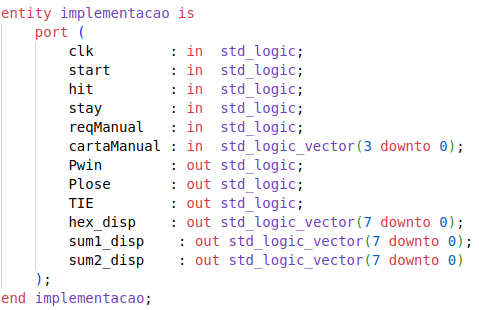
\includegraphics[width=0.9\linewidth]{top_blackjack.png}
    \caption{Entidade top level do problema}
    \label{fig:top_entity}
\end{figure}

Na top level criada, os mesmos clock e reset/start são divididos para as FSM\ref{tab:geradorcarta} e FSM\ref{tab:blackjack}. hit e stay são entradas de Blackjack, reqManual e cartaManual são entradas do gerador de cartas. As saídas da top-level são todas da FSM\ref{tab:blackjack}, os sinais de reqCard e a carta gerada pela FSM\ref{tab:geradorcarta} são controlados por meio de signals declarados na arquitetura da top-level. A partir dessa entidade, fizemos o mapeamento para a implementação na FPGA que se deu da seguinte maneira: 

\begin{table}[H]
    \centering
    \begin{tabular}{|c|c|}
    \hline
        variáveis VHDL & mapeamento FPGA \\
        \hline        
        clk & KEY(0) \\
        \hline
        reset / start & KEY(1) \\
        \hline
        SW(1) & stay \\
        \hline 
        SW(5) & reqManual \\
        \hline
        SW(0) & hit \\
        \hline
        SW(9), SW(8), SW(7), SW(6) & cartaManual \\
        \hline
        LEDR(0) & Plose \\
        \hline
        LEDR(1) & TIE \\
        \hline
        LEDR(2) & Pwin \\
        \hline
        HEX0 & sum1disp\\
        \hline
        HEX1 & sum2disp\\
        \hline
        HEX3 & hexdisp\\
        \hline
    \end{tabular}
    \caption{Mapeamento na placa FPGA}
    \label{tab:mapeamento}
\end{table}



\chapter{Notas e considerações finais}
O presente trabalho funciona para os cenários de solicitar e receber uma carta, atualizar corretamente os valores da mão do jogador e carteador. O código lida com a possibilidade de valores do Ás (decide de forma inteligente se deve somá-lo como 11 ou 1), lida com as possibilidades de estouro com e sem ás, partindo de qualquer tipo de valor de carta recebido, e exibe corretamente nos LEDs correspondentes o resultado da rodada jogada.

A projeção da segunda máquina de estados seguiu à risca as recomendações dadas pelo problema, ciente das limitações apresentadas para a execução do jogo na FPGA, onde principalmente os displays são limitados, fazendo com que haja a necessidade de jogar completamente a rodada do jogador e só depois de haver um STAY, isto é, o jogador escolhe terminar sua vez sem que tenha estourado o limite da soma em 21, é que se começa a jogada do dealer. Dessa forma, uma vez que o jogador estoura, o carteador sempre vence. 

Para melhor legibilidade visual, abstraímos os estados dummies do problema que funcionam da seguinte maneira: um estado genérico solicita uma carta e transita para um estado dummy correspondente. Dentro desse estado, ele fica em espera enquanto a carta estiver inválida (0000). Quando a carta é corretamente recebida e interpretada pelo sistema, ele transita para um novo estado de soma correspondente, onde serão feitas alterações nos valores de jogador e dealer de acordo com a situação.

A arquitetura de Blackjack não lida com a possibilidade de receber uma carta inválida, isto é, a entrada '0000' ao enviar o sinal de reqManual. Quando um sinal de reqManual é enviado com o sinal inválido no input, a máquina entra em um estado de loop pois ela permanece no estado dummy até que a carta seja diferente de 0, o que não irá acontecer já que o sinal de req é colocado em 0 na transição para o estado dummy.
\end{document}
 